
\documentclass{beamer}


\mode<presentation>
{
  \usetheme{Hawke}
  \setbeamercovered{transparent}
}


\usepackage[english]{babel}
% or whatever

\usepackage[latin1]{inputenc}
% or whatever

\usepackage{times}
\usepackage[T1]{fontenc}
% Or whatever. Note that the encoding and the font should match. If T1
% does not look nice, try deleting the line with the fontenc.

\usepackage{multimedia}


%%%%%%
% My Commands
%%%%%%

\newcommand{\ml}{{\sc matlab}}
\newcommand{\bb}{{\boldsymbol{b}}}
\newcommand{\bx}{{\boldsymbol{x}}}
\newcommand{\by}{{\boldsymbol{y}}}
\newcommand{\bfm}[1]{{\boldsymbol{#1}}}

%%%%

\title[Lecture 5] % (optional, use only with long paper titles)
{Lecture 5 - Iterative Methods}

% \subtitle
% {Include Only If Paper Has a Subtitle}

\author[I. Hawke] % (optional, use only with lots of authors)
{I.~Hawke}
% - Give the names in the same order as the appear in the paper.
% - Use the \inst{?} command only if the authors have different
%   affiliation.

\institute[University of Southampton] % (optional, but mostly needed)
{
%  \inst{1}%
  School of Mathematics, \\
  University of Southampton, UK
}
% - Use the \inst command only if there are several affiliations.
% - Keep it simple, no one is interested in your street address.

\date[Semester 1] % (optional, should be abbreviation of conference name)
{MATH3018/6141, Semester 1}
% - Either use conference name or its abbreviation.
% - Not really informative to the audience, more for people (including
%   yourself) who are reading the slides online

\subject{Numerical methods}
% This is only inserted into the PDF information catalog. Can be left
% out.



% If you have a file called "university-logo-filename.xxx", where xxx
% is a graphic format that can be processed by latex or pdflatex,
% resp., then you can add a logo as follows:

\pgfdeclareimage[height=0.5cm]{university-logo}{mathematics_7469}
\logo{\pgfuseimage{university-logo}}



% Delete this, if you do not want the table of contents to pop up at
% the beginning of each subsection:
%  \AtBeginSubsection[]
%  {
%    \begin{frame}<beamer>
%      \frametitle{Outline}
%      \tableofcontents[currentsection,currentsubsection]
%    \end{frame}
%  }
\AtBeginSection[]
{
  \begin{frame}<beamer>
    \frametitle{Outline}
    \tableofcontents[currentsection]
  \end{frame}
}


% If you wish to uncover everything in a step-wise fashion, uncomment
% the following command:

%\beamerdefaultoverlayspecification{<+->}


\begin{document}

\begin{frame}
  \titlepage
\end{frame}

\section{Iterative Methods}

\subsection{Iterative Methods}

\begin{frame}
  \frametitle{Iterative Methods}

   We (still) want to solve the linear system
   \begin{equation*}
     A \bx = \bb.
   \end{equation*}
   All direct methods require ${\cal O}(n^3)$ operations. For large
   matrices this takes time and each operation introduces error that
   may accumulate. Other methods may be preferable. \pause

   \vspace{1ex}

   Iterative methods build a \emph{sequence} of approximate
   solutions. Start from ``guess'' $\bx^{(0)}$ and compute
   approximations $\bx^{(1)}, \bx^{(2)}, \dots, \bx^{(N)}$ which
   converge to the exact solution.

   \vspace{1ex}

   Sequence can be truncated to save time or when solution found to
   sufficient accuracy. \pause

   \vspace{1ex}

   Key elements of an iterative method:
   \begin{enumerate}
   \item A rapid convergence to the correct solution,
   \item A fast algorithm for computing each successive approximation.
   \end{enumerate}

\end{frame}

\begin{frame}
  \frametitle{A general framework}

  Standard ``notation'' is to split the matrix as
  \begin{equation*}
    A = N - P,
  \end{equation*}
  where $N$ and $P$ are (as yet unknown) $n \times n$ matrices.
  The linear system becomes
  \begin{equation*}
    N \bx = P \bx + \bb.
  \end{equation*} \pause

  Then \emph{assume} that we have an approximate solution, or guess,
  $\bx^{(0)}$, and define the sequence
  \begin{equation*}
    N \bx^{(i)} = P \bx^{(i - 1)} + \bb, \quad i = 1, 2, \dots
  \end{equation*} \pause

  Obviously consistent with the original equation.  The algorithm will
  only be useful if
  \begin{enumerate}
  \item $N$ is nonsingular, and
  \item The linear system $N \bfm{y} = \bfm{z}$ is ``easy'' to solve.
  \end{enumerate}

\end{frame}


\subsection{Convergence}

\begin{frame}
  \frametitle{Convergence}

  To work, the sequence
  \begin{equation*}
    \bx^{(i)} = N^{-1} \left( P \bx^{(i - 1)} + \bb \right), \quad i =
    1, 2, \dots
  \end{equation*}
  must have a limit.  Intuitively clear that the matrix $M =
  N^{-1} P$ is central to the convergence or otherwise of
  this sequence.

  \vspace{1ex}

  {\bf Theorem}: The iterative method described converges if and only
  if $M = N^{-1} P$ exists and
  \begin{equation*}
    \varrho (M) \equiv \max_i | \lambda_i | < 1.
  \end{equation*}

  \begin{overlayarea}{\textwidth}{0.3\textheight}
    \only<2|handout:0>
    {
      View $\bx^{(i)}$ as a vector in $n$-dimensional space: ensures
      that repeatedly multiplying by $M$ does not cause result to
      diverge.
    }
    \only<3>
    {
      The \emph{spectral radius} $\varrho (M)$ can be hard
      to compute. Often use the weaker condition
      \begin{equation*}
        \| M \| < 1 \Rightarrow \text{Method converges}.
      \end{equation*}
    }
  \end{overlayarea}

\end{frame}


\subsection{Jacobi's Method}

\begin{frame}
  \frametitle{General assumptions}

  \vspace{2ex}

  In what follows we shall always assume that all diagonal entries are
  1. \pause

  \vspace{2ex}

  If this is not true, we can always arrange it to be so by dividing
  each row by its diagonal element. \pause

  \vspace{2ex}

  If the diagonal element of any row is zero, permute the rows. It
  must be possible to arrange a \emph{nonsingular} matrix such that
  every diagonal element is non-zero just by row operations.

\end{frame}

\begin{frame}
  \frametitle{Jacobi's Method}

  One key requirement on the split
  \begin{equation*}
    A = N - P
  \end{equation*}
  was that the $N \bfm{y} = \bfm{z}$ should be easy to solve. The
  simplest possible problem would be $N = I$. \pause

  \vspace{1ex}

  This means (as $A$ is 1 on the diagonal) that
  \begin{equation*}
    P = A_L + A_U
  \end{equation*}
  where $A_L$ and $A_U$ are the ``triangular'' parts of $-A$ (note
  sign!). The iteration scheme is
  \begin{equation*}
    \bx^{(i)} =  (A_L + A_U) \bx^{(i - 1)} + \bb, \quad i = 1, 2, \dots
  \end{equation*}
  and the convergence matrix is $M = P$.

\end{frame}

\begin{frame}
  \frametitle{Example of Jacobi's Method}

  We look at the solution of the simple linear system
  \begin{equation*}
    \begin{pmatrix}
      3 & 1 \\
      1 & 3
    \end{pmatrix}
    \begin{pmatrix}
      x_1 \\ x_2
    \end{pmatrix} =
    \begin{pmatrix}
      5 \\ 7
    \end{pmatrix}
  \end{equation*}
  using Jacobi's Method. \pause  Ensure the diagonal
  elements are all 1:
  \begin{equation*}
    A =
    \begin{pmatrix}
      1 & \tfrac{1}{3} \\
      \tfrac{1}{3} & 1 \\
    \end{pmatrix},
    \quad \bb =
    \begin{pmatrix}
      \tfrac{5}{3} \\ \tfrac{7}{3}
    \end{pmatrix}.
  \end{equation*} \pause
  Check convergence by computing
  \begin{equation*}
    M = P =
    \begin{pmatrix}
      0 & -\tfrac{1}{3} \\
      -\tfrac{1}{3} & 0
    \end{pmatrix}
  \end{equation*}
  which implies, as $\varrho(M) = 1 / 3 < 1$, that the method will
  converge.

\end{frame}

\begin{frame}
  \frametitle{Example of Jacobi's Method 2}

  \begin{columns}
    \begin{column}{0.475\textwidth}
      The sequence has entries
      \begin{tabular}{|c|c c|}
        $i$ & $x_1$ & $x_2$ \\ \hline
        $0$ & $0$ & $0$ \\
        $1$ & $5 / 3$ & $7 / 3$ \\
        $2$ & $0.888889$ & $1.777778$ \\
        $5$ & $1.008230$ & $2.004115$ \\
        $10$ & $0.999983$ & $1.999966$ \\
        $100$ & $1.000000$ & $2.000000$
      \end{tabular}
    \end{column}
    \begin{column}{0.525\textwidth}
      \begin{center}
        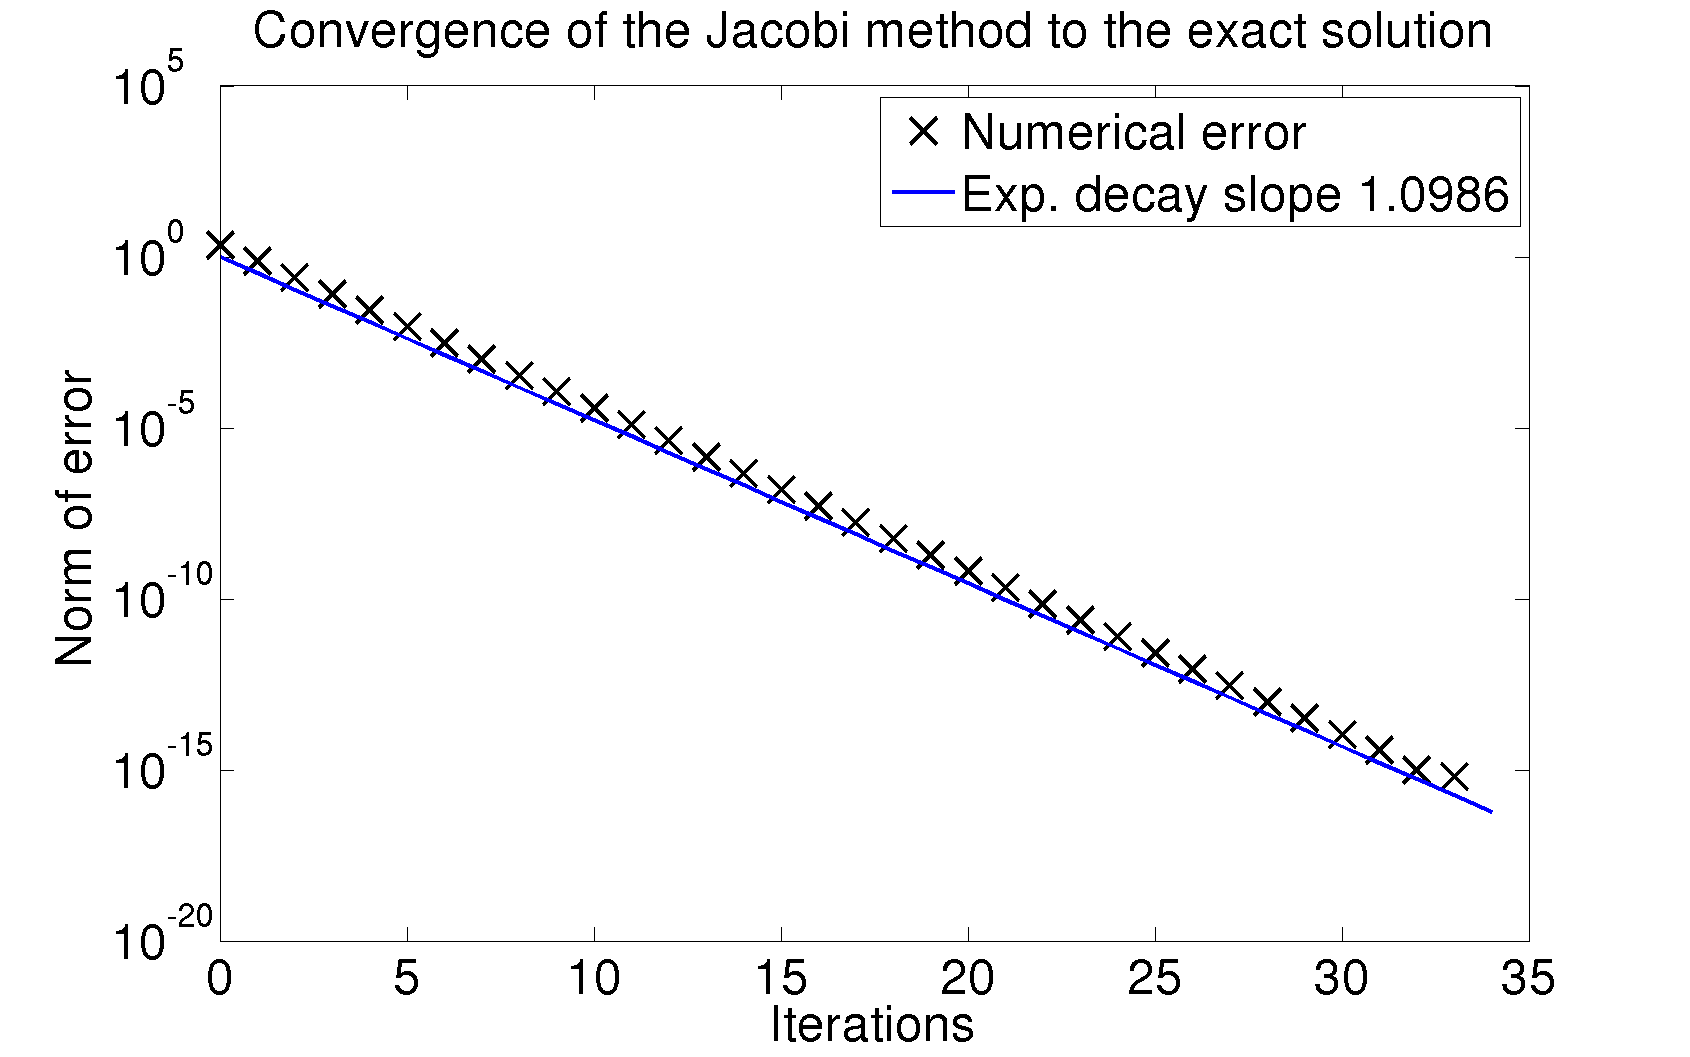
\includegraphics[width=\textwidth]{figures/Jacobi1}
      \end{center}
    \end{column}
  \end{columns}

  \vspace{1ex}

  A starting ``guess'' of $\bx = \bfm{0}$ appears to converge to $\bx
  = (1, 2)^T$. The convergence is exponential with a slope $\sim 1$.

\end{frame}


\subsection{Gauss-Seidel Method}

\begin{frame}
  \frametitle{Gauss-Seidel Method}

  In the Gauss-Seidel method split the coefficient matrix as
  \begin{equation*}
    A = I - (A_L + A_U)
  \end{equation*}
  as before. Choose
  \begin{align*}
    N & = I - A_L, \\
    P & = A_U.
  \end{align*}
  This makes the iteration scheme
  \begin{equation*}
    \bx^{(i)} =  A_L \bx^{(i)} + A_U \bx^{(i - 1)} + \bb, \quad i = 1,
    2, \dots
  \end{equation*} \pause

  Written in this form as $A_L$ \emph{strictly} lower
  triangular. Consider each component of the iteration scheme from the
  top down: each coefficient of $\bx^{(i)}$ is computed on the left
  before it is used on the right.

\end{frame}

\begin{frame}
  \frametitle{Example of Gauss-Seidel Method}

  As above we look at
  \begin{equation*}
    \begin{pmatrix}
      3 & 1 \\
      1 & 3
    \end{pmatrix}
    \begin{pmatrix}
      x_1 \\ x_2
    \end{pmatrix} =
    \begin{pmatrix}
      5 \\ 7
    \end{pmatrix} \rightarrow
    \begin{pmatrix}
      1 & \tfrac{1}{3} \\
      \tfrac{1}{3} & 1 \\
    \end{pmatrix}
    \begin{pmatrix}
      x_1 \\ x_2
    \end{pmatrix} =
    \begin{pmatrix}
      \tfrac{5}{3} \\ \tfrac{7}{3}
    \end{pmatrix}.
  \end{equation*}
  We have
  \begin{equation*}
    A_L =
    \begin{pmatrix}
      0 & 0 \\
      -1/3 & 0
    \end{pmatrix}, \quad
    A_U =
    \begin{pmatrix}
      0 & -1/3 \\
      0 & 0
    \end{pmatrix}
  \end{equation*}
  and hence the iteration algorithm becomes
  \begin{align*}
    \begin{pmatrix}
      x_1^{(i)} \\ x_2^{(i)}
    \end{pmatrix} & = \frac{1}{3} \left[
      \begin{pmatrix}
        -x_2^{(i-1)} \\ - x_1^{(i)}
      \end{pmatrix} +
      \begin{pmatrix}
        5 \\ 7
      \end{pmatrix} \right]
    = \frac{1}{3}
    \begin{pmatrix}
      5 - x_2^{(i-1)} \\ 7 - x_1^{(i)}
    \end{pmatrix}.
  \end{align*}
  If read row-by-row from the top we have always computed the
  $\bx^{(i)}$ entries before they are used.

\end{frame}


\begin{frame}
  \frametitle{Example of Gauss-Seidel Method 2}

  \begin{columns}
    \begin{column}{0.475\textwidth}
      The sequence has entries
      \begin{tabular}{|c|c c|}
        $i$ & $x_1$ & $x_2$ \\ \hline
        $0$ & $0$ & $0$ \\
        $1$ & $5 / 3$ & $16 / 9$ \\
        $2$ & $1.074074$ & $1.975309$ \\
        $5$ & $1.000102$ & $1.999966$ \\
        $10$ & $1.000000$ & $2.000000$ \\
        $100$ & $1.000000$ & $2.000000$
      \end{tabular}
    \end{column}
    \begin{column}{0.525\textwidth}
      \begin{center}
        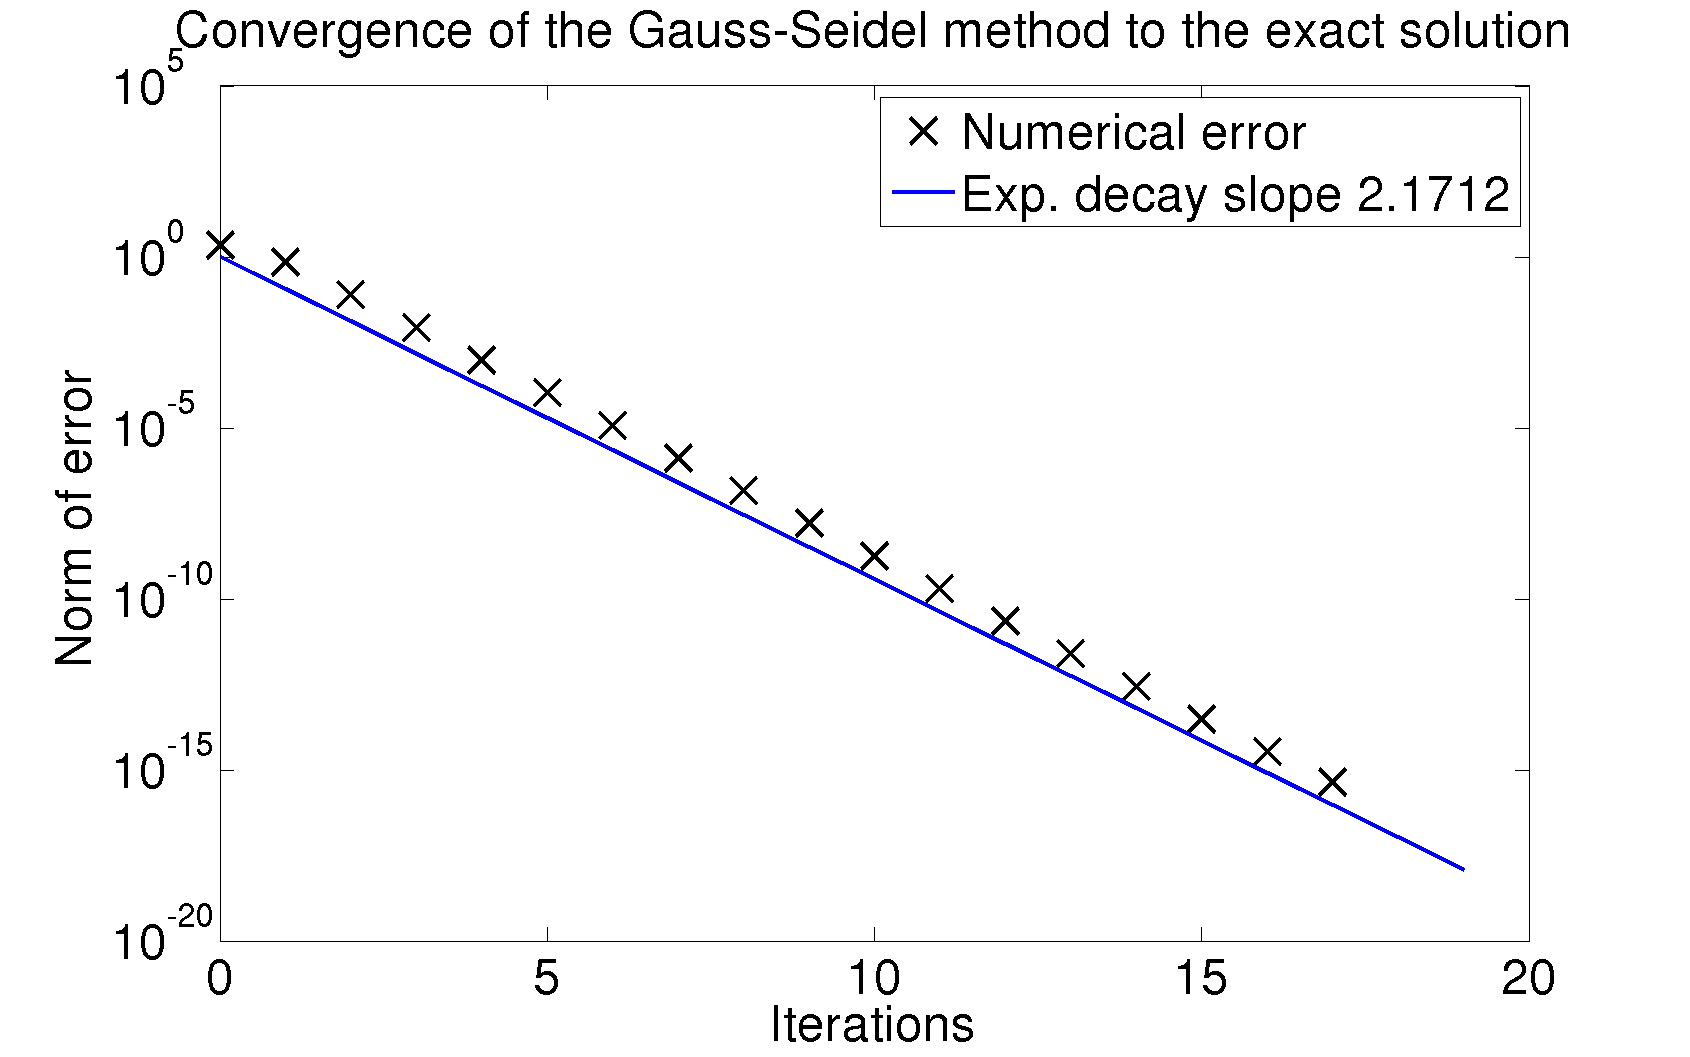
\includegraphics[width=\textwidth]{figures/GaussSeidel1}
      \end{center}
    \end{column}
  \end{columns}

  \vspace{1ex}

  A starting ``guess'' of $\bx = \bfm{0}$ appears to converge to $\bx
  = (1, 2)^T$. The convergence is exponential with a slope $\sim 2$,
  much faster than Jacobi's Method.

\end{frame}


\subsection{Successive Over Relaxation}

\begin{frame}
  \frametitle{Successive Over Relaxation}

  View the sequence as repeated ``corrections'' to the previous term,
  \begin{equation*}
    \bx^{(i)} = \bx^{(i-1)} + \bfm{c},
  \end{equation*}
  where correction is based e.g.\ on Gauss-Seidel method,
  \begin{equation*}
    \bfm{c} = A_L \bx^{(i)} + (A_U - I) \bx^{(i-1)} + \bb.
  \end{equation*} \pause

  Modify correction by factor $\omega$:
  \begin{equation*}
    \bx^{(i)} = \bx^{(i-1)} + \omega \bfm{c}.
  \end{equation*} \pause

  \emph{A priori} best value of $\omega$ not clear.  Typically it is
  set close to one. However, poor choices may cause the algorithm to
  diverge!

\end{frame}


\begin{frame}
  \frametitle{Example of SOR Method 1}

  \begin{columns}
    \begin{column}{0.475\textwidth}
      Solving the previous example using $\omega = 1.035$, the
      sequence has entries
      \begin{tabular}{|c|c c|}
        $i$ & $x_1$ & $x_2$ \\ \hline
        $0$ & $0$ & $0$ \\
        $1$ & $1.725000$ & $1.819875$ \\
        $2$ & $1.036768$ & $1.993619$ \\
        $5$ & $0.999999$ & $2.000000$ \\
        $10$ & $1.000000$ & $2.000000$ \\
        $100$ & $1.000000$ & $2.000000$
      \end{tabular}
    \end{column}
    \begin{column}{0.525\textwidth}
      \begin{center}
        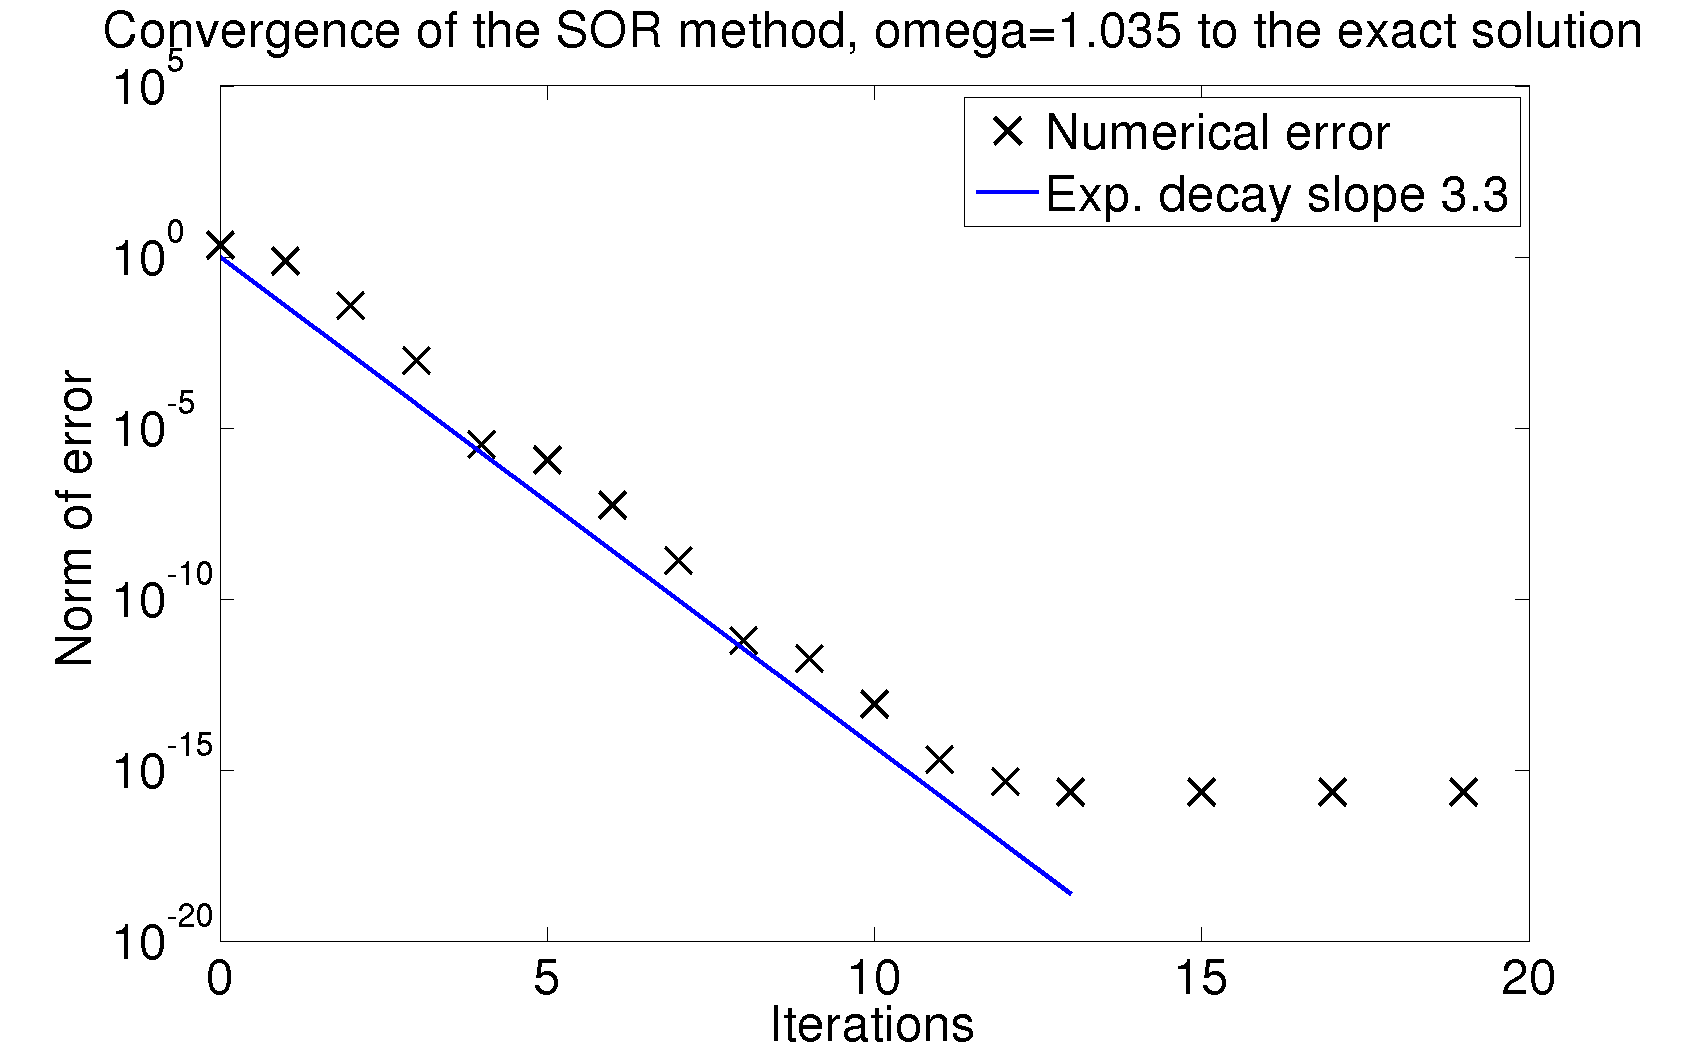
\includegraphics[width=\textwidth]{figures/SOR1}
      \end{center}
    \end{column}
  \end{columns}

  \vspace{1ex}

  A starting ``guess'' of $\bx = \bfm{0}$ appears to converge to $\bx
  = (1, 2)^T$. The convergence is exponential with a slope $\sim 3$,
  the fastest method so far.

\end{frame}

\begin{frame}
  \frametitle{Example of SOR Method 2}

  \begin{columns}
    \begin{column}{0.475\textwidth}
      Solving the previous example using $\omega = 1.2$, the
      sequence has entries
      \begin{tabular}{|c|c c|}
        $i$ & $x_1$ & $x_2$ \\ \hline
        $0$ & $0$ & $0$ \\
        $1$ & $2.000000$ & $2.000000$ \\
        $2$ & $0.800000$ & $2.080000$ \\
        $5$ & $0.998221$ & $2.000430$ \\
        $10$ & $1.000000$ & $2.000000$ \\
        $100$ & $1.000000$ & $2.000000$
      \end{tabular}
    \end{column}
    \begin{column}{0.525\textwidth}
      \begin{center}
        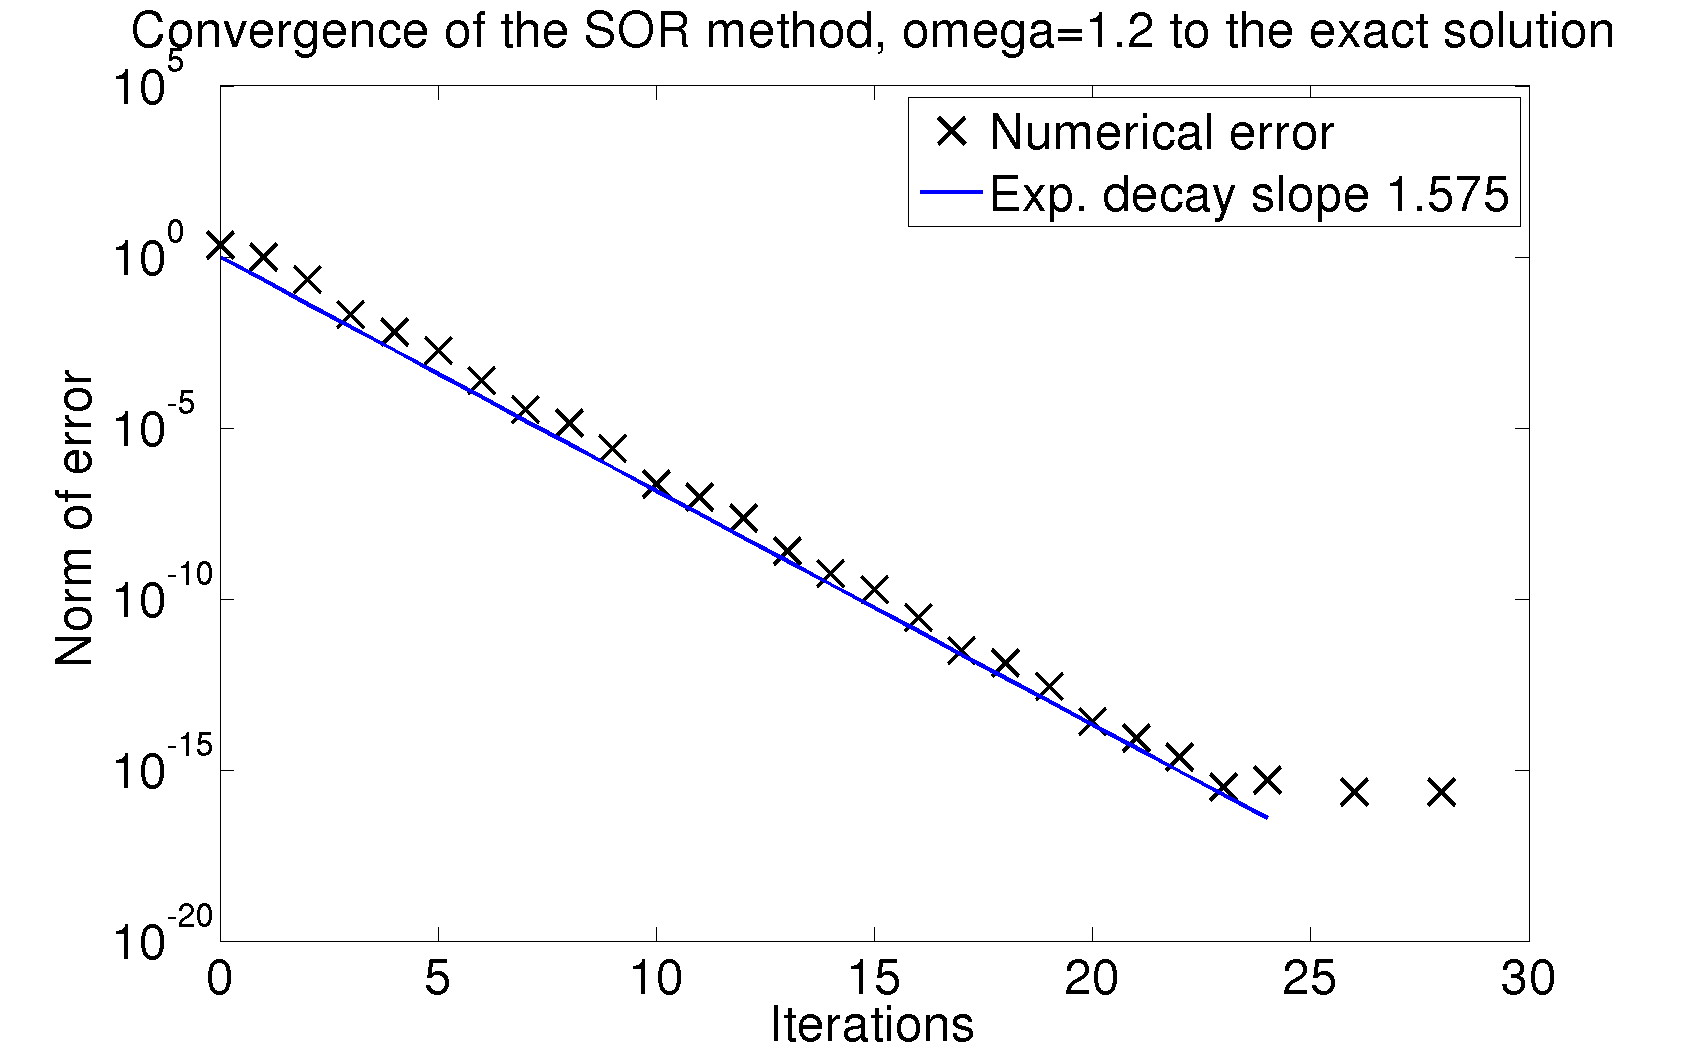
\includegraphics[width=\textwidth]{figures/SOR2}
      \end{center}
    \end{column}
  \end{columns}

  \vspace{1ex}

  A starting ``guess'' of $\bx = \bfm{0}$ appears to converge to $\bx
  = (1, 2)^T$. The convergence is exponential with a slope $\sim 1.6$,
  which is not as good as Gauss-Seidel.

\end{frame}

\begin{frame}
  \frametitle{The relaxation parameter}

  \begin{center}
    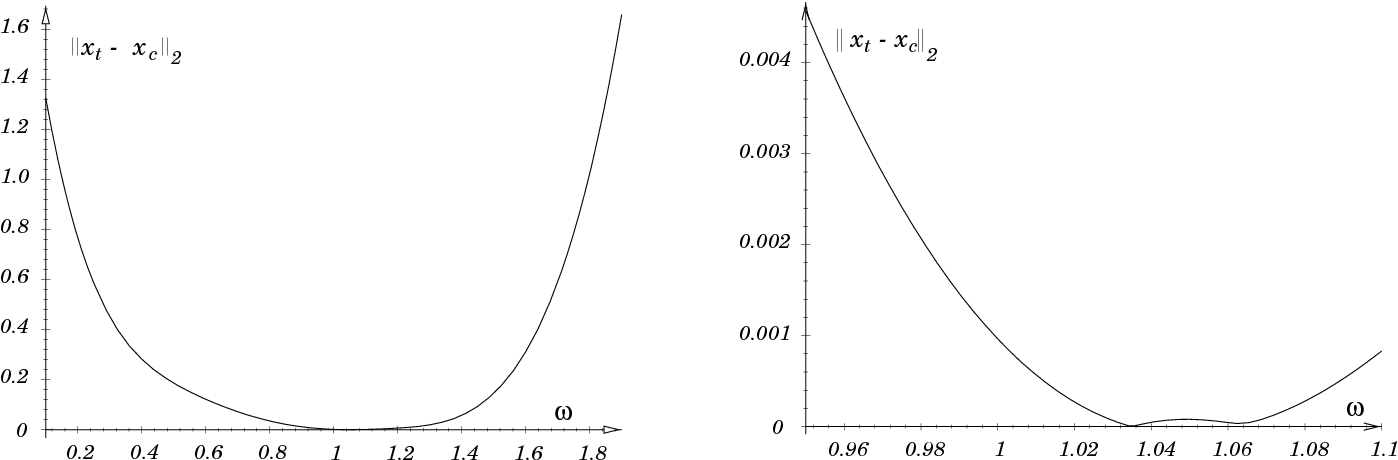
\includegraphics[width=0.9\textwidth]{figures/SOR}
  \end{center}
  The norm of the error obtained with SOR after four iterations.  The
  convergence behaviour depends in a highly non-trivial way on
  $\omega$.

  \vspace{1ex}

  SOR algorithms are much harder to analyze than Jacobi or
  Gauss-Seidel.

\end{frame}


\subsection{Convergence Analysis}

\begin{frame}
  \frametitle{Convergence analysis}

  Two theorems about \emph{when} these methods will work:

  \vspace{2ex}

  {\bf Theorem 1}: If the coefficient matrix $A$ is \emph{strictly}
  diagonally dominant then both the Jacobi method and the Gauss-Seidel
  method will converge.

  \vspace{2ex}

  {\bf Theorem 2}: If the coefficient matrix $A$ is symmetric and
  positive definite then the Gauss-Seidel method will converge.

\end{frame}


\section{Other matrix operations}


\subsection{Other matrix operations}

\begin{frame}
  \frametitle{Other matrix operations}

  We have so far only considered the linear system
  \begin{equation*}
    A \bx = \bb.
  \end{equation*}
  We have given methods to solve this system accurately without
  computing the matrix inverse or determinant. However, these methods
  can also be used to efficiently and accurately compute these
  quantities.
\end{frame}

\begin{frame}
  \frametitle{Determinants}

  Given the $LU$ decomposition we have
  \begin{equation*}
    \det (A) = \det(L) \times \det(U), \quad \text{and} \quad \det(U)
    = \prod_{i=1}^n u_{ii}.
  \end{equation*}
  Choose $\ell_{ii}=1$ giving $\det(L) = 1$: determinant
  follows. \pause

  \vspace{1ex}

  Similarly Gaussian elimination with partial pivoting gives
  \begin{equation*}
    \det(A) = \pm \prod_{i=1}^n u_{ii},
  \end{equation*}
  where the sign depends on the number of row swaps performed.\pause

  \vspace{1ex}

  {\bf Note:} Gaussian elimination, and hence finding the determinant,
  is an ${\cal O}(n^3)$ operation.  The expansion in minors is an
  ${\cal O}(n!)$ operation.

\end{frame}

\begin{frame}
  \frametitle{Matrix inversion}

  Solving for the matrix inverse can be written as a set of linear
  system problems. We write
  \begin{equation*}
    A A^{-1} = I
  \end{equation*}
  and consider each column of $A^{-1}$ as a separate problem. \pause
  Writing $\bfm{c}_i$ for the (unknown) column of $A^{-1}$ we have
  \begin{equation*}
    A \bfm{c}_i =
    \begin{pmatrix}
       \vdots \\ 0 \\ 1 \\ 0 \\ \vdots
    \end{pmatrix}
  \end{equation*}
  where the $1$ appears in the $i^{\text{th}}$ row. \pause

  \vspace{1ex}

  This finds the inverse by solving $n$ linear systems, which is much
  faster than evaluating the $n+1$ determinants required by Cramer's
  rule.

\end{frame}

\section{Summary}

\subsection{Summary}

\begin{frame}
  \frametitle{Summary}

  \begin{itemize}
  \item Iterative methods are often based on the split
    \begin{equation*}
      A = N - P.
    \end{equation*}
  \item Convergence depends on $M = N^{-1}P$.
  \item Jacobi chooses $N = I$ and converges slowly.
  \item Gauss-Seidel chooses $N = I - A_U$ and uses coefficients as
    soon as they become available. Slightly harder to code, it
    converges faster than Jacobi.
  \item SOR tries to ``accelerate'' the convergence of Gauss-Seidel
    depending on a parameter $\omega$. It can be faster, but the
    behaviour depends non-trivially on $\omega$ and it is very
    difficult to analyze.
  \item Strict diagonal dominance is sufficient for convergence of
    both Jacobi and Gauss-Seidel methods.
  \item Computing determinants and inverses from the solution of
    linear systems is usually much faster than ``standard''
    techniques.
  \end{itemize}

\end{frame}

\end{document}



%%% Local Variables:
%%% mode: latex
%%% TeX-master: t
%%% End:
